\chapter{Background and related work}
\section{SDN and OpenFlow}
OpenFlow is the most popular southbound interface in SDN. A switch that supports OpenFlow is called an OpenFlow switch. Aside from physical switches, there are also software implementations of virtual switches, such as \textit{Open vSwtich} (\url{openvswitch.org}). OpenFlow switches typically separate OpenFlow and non-OpenFlow traffic, which do not interfere with each other \cite{HP_SPEC}.

A controller is able to determine the forwarding path of packets by adding, updating and deleting flow entries in the flow tables of OpenFlow switches in both reactive and proactive ways \cite{OF_SPEC}. It also maintains the abstract view of the network, including network topology, host positions and the states of network resources. An incoming packet from the \textit{ingress port} will go through one or more flow tables, optionally through the group table, and be processed according to the actions defined by the matched flow entry. Each OpenFlow table typically contains thousands of flow entries. Figure~\ref{FE_Col} presents the columns of a flow entry. Packets will be matched with the \textit{match fields} of a flow entry. When a packet matches a flow entry, the action set to that packet will be modified according to the instructions in the entry. There is an entry with the lowest priority that matches all fields. It is for packets that cannot match any other flow entries. Normally, such a packet will be encapsulated and sent to the controller, which will decide how to process it and add a new flow entry according to the network policy. After the end of processing pipeline, the actions in the action set will be executed.% When ports are added or removed, the content of flow tables remain unchanged, so the controller should clean up the reference of a port if a port is deleted \cite{OF_SPEC}.

\begin{figure}[H]
\begin{center} 
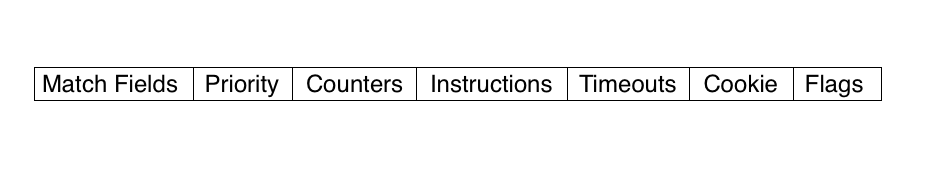
\includegraphics[width=1\textwidth]{figures/columns_of_flow_entry.png}
\end{center}
\caption{Columns of a flow entry.}
\label{FE_Col}
\end{figure}

\section{Topology discovery services}
\label{Topology discovery services}
The controller needs to maintain the visibility of the whole network to realize centralized control and high programmability. Therefore, topology discovery services play an important role in SDN. The services help to reduce manual efforts significantly when the topology is altered. The topology services include three parts: switch discovery, host tracking and internal link.

\subsection{Switch discovery service and Host tracking service}
Switch discovery is rather simple. When a switch initiates a connection with a controller, the OpenFlow channel will be established, and the switch information will be sent to the controller. A controller maintains the host profiles to keep track of the locations of hosts. When a packet-miss happens in the flow table, a \texttt{Packet\_In} message will be sent to the controller along with the packet's information and the controller will look up the host profiles it maintains. If the host profile of the host cannot be found, the controller will assume a new host joining the network and add the information of the host. If there is a conflict between the host profile and the \texttt{Packet\_In} message, the controller treats this as a host migration and updates the location in the host profile.

\subsection{Link discovery service}
\label{Link discovery service}
Link discovery refers to the procedure of discovering the links between switches. Since there has not been a standard for the link discovery in the OpenFlow controller, we will use the term \textit{OpenFlow Discovery Protocol} (OFDP) when mentioning it. Currently, all mainstream controllers support OFDP despite some minor differences in detail.

OFDP leverages the Link Layer Discovery Protocol (LLDP) with subtle modification to perform topology discovery in an OpenFlow network. LLDP is originally implemented for an Ethernet switch to exchange its identity and capabilities with adjacent layer-2 peers. In a legacy network, LLDP packets are sent regularly via each port of switches \cite{LLDP_WS}. A switch stores the information learned from LLDP packets sent by the neighbors and the packets will not be forwarded further. Figure~\ref{LLDP_frame} shows the structure of an LLDP Ethernet frame. Each LLDP data unit contains a sequence of type-length-values (TLV). 

\begin{figure}[H]
\begin{center} 
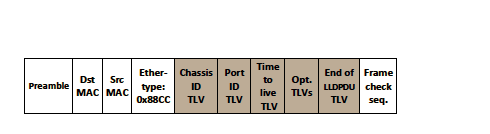
\includegraphics[width=1\textwidth]{figures/LLDP_packet_format.png}
\end{center}
\caption{LLDP packet frame structure. \cite{LLDP_WS}}
\label{LLDP_frame}
\end{figure}

However, OFDP operates quite differently. The controller keeps the topology information, and an OpenFlow switch does nothing more than forwarding the LLDP packet. The simplified process is shown in Figure~\ref{OFDP}. All switches have a pre-installed rule in their flow tables. The rule specifies to send LLDP packets received from any ports except the controller port back to controller via \texttt{Packet\_In}. Initially, the controller creates an LLDP packet for each port on every switch via the \texttt{Packet\_Out} message. After receiving the LLDP packet from controller, S1 sends it out on Port 1 and received by S2 on Port 3. With the pre-installed forwarding rule, switch S2 forwards the received LLDP packet to the controller via a \texttt{Packet\_In} message, which contains meta-data such as the identifier of the switch and the ingress port via which the packet was received. Thus, the controller can now infer that there exists a link between Port 1 of S1 and Port 3 of S2, and this information will be added to controller's topology database. After running this process through all the ports on all the switches, the controller will obtain all links between switches in the network. The entire discovery process is performed periodically with a typical default interval size of 5 seconds \cite{PPTI14}. 

\begin{figure}[H]
\begin{center} 
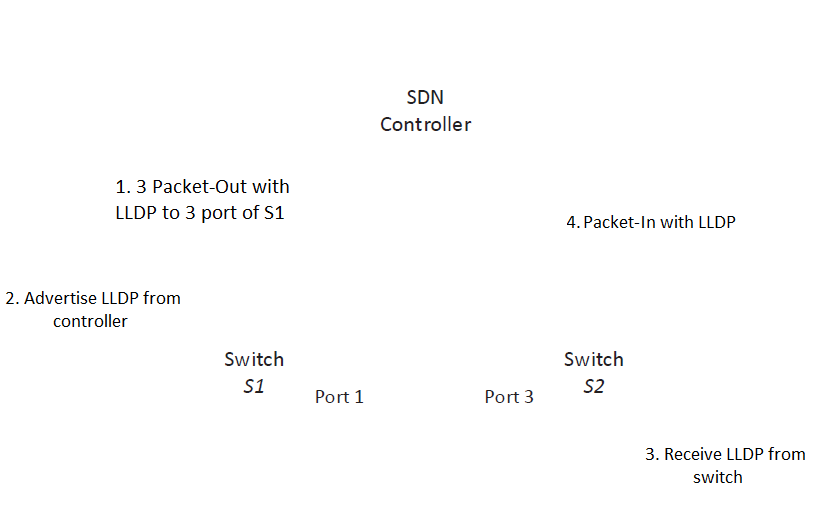
\includegraphics[width=1\textwidth]{figures/OFDP_procedure.png}
\end{center}
\caption{An illustration of OFDP procedure.}
\label{OFDP}
\end{figure}

\section{SDN security}
\label{SDN security}
A thorough review of SDN-related security issues can be found in \cite{LAB14, CM, SOS13, KJK}. Therefore, rather than repeat the review, we will focus on the issue of compromising OpenFlow switches, since it has been less addressed than others so far. Compromising OpenFlow switches can lead to some bad results. (1) Attacker may launch topology poisoning attack by manipulating link discovery packet. (2) The actions specified in the flow rules on a compromised switch can be unexpectedly altered. (3) The packets through a compromised switch can be eavesdropped or dropped. (4) The compromised switch may be configured to be managed by another malicious controller. (5) It is possible to launch network-wide DOS attack by sending specific forged packet to consume the controller's resource.

The main idea of the topology poisoning attack is to trick the controller into believing the existence of a non-existing link to host or switch by exploiting traits of topology management service. One can initiate such type of attack with either a switch or a host. In \cite{HXWG15}, Hong et al. mentioned Host Location Hijacking Attack and Link Fabrication Attack, and presented TopoGuard to solve the problem. However, LLDP packets are passed around with the aid of switches. The Link Fabrication Attack can be also initiated by compromised switches, but the attack vector  is not covered in the scenario of TopoGuard. Bui gives three different attack scenarios of Link Fabrication Attack with compromised switches and evaluates their consequence under different routing algorithms and network topologies \cite{TTB15}. This attack is caused by the lack of authentication of LLDP. However, simply adding authenticator inside the LLDP packet will not help against LLDP relay attack \cite{HXWG15}. Alharbi et al. implement HMAC based mechanism with a little modification to static secret key, which is able to detect the injection of any fabricated LLDP packets, with only an acceptable of amount of overhead added \cite{ATPP15}.

Attackers can also modify the flow entries inside the flow tables of the compromised switch to perform MITM, eavesdropping or DOS attack \cite{AAS14}. The detection method proposed in \cite{CKGL15} is able to detect whether a switch is forwarding the packets in an unexpected way. After selecting a flow entry as the detecting target, they install new entry on its neighbors. With the match field selected by their algorithm, they are able to let every packet that matches the new flow entry matches the target flow entry. A packet containing the match field of the new flow entry will be sent from \texttt{Packet\_Out} to a neighbor of the target switch, forwarded to the target switch, and should be sent back to the controller. Finally, they will check if the packet comes back to the controller as expected and remain unchanged. However, this method will take a long time to run if it is desired to scan through a large number of flow entries. A pre-detection method to narrow down the potential target is needed.